%! Integrantes:
%! Andre Gilmer Santos Felix (Matemática)
%! Leon Alonzo Terrones Caccha (Matemática)
%! Carlos Alonso Aznarán Laos (Matemática)
%! Universidad Nacional de Ingeniería
%! Facultad de Ciencias
%! Lima, Perú
%! Uso:
%! $ sudo pacman -Syu texlive texlive-langspanish zathura # dependencias, visor
%! $ chmod +x run.sh
%! $ ./run.sh
%! Ver https://wiki.archlinux.org/title/TeX_Live
% arara: clean: {
% arara: --> extensions:
% arara: --> ['aux','bbl','bcf','blg','log','nav','out',
% arara: --> 'pdf','run.xml','snm','synctex.gz','toc']      
% arara: --> }
% arara: lualatex: {
% arara: --> shell: yes,
% arara: --> draft: yes,
% arara: --> interaction: batchmode
% arara: --> }
% arara: biber
% arara: lualatex: {
% arara: --> shell: yes,
% arara: --> draft: yes,
% arara: --> interaction: batchmode
% arara: --> }
% arara: lualatex: {
% arara: --> shell: yes,
% arara: --> synctex: yes,
% arara: --> interaction: batchmode
% arara: --> }
% arara: clean: {
% arara: --> extensions:
% arara: --> ['aux','bbl','bcf','blg','log','nav','out',
% arara: --> 'run.xml','snm','synctex.gz','toc']
% arara: --> }
\PassOptionsToPackage{svgnames}{xcolor}
\documentclass[
	spanish,
	8pt,
	xcolor=table,
	handout,
	aspectratio=1610,
	professionalfonts,
	% notheorems,
	mathserif,
	leqno,
	% t
]{beamer}
\setbeamersize{text margin left=5pt,text margin right=5pt}
\usepackage[spanish,es-sloppy]{babel}
\spanishdatedel\decimalpoint
\usepackage{mathtools}
% \usepackage{minted}
\usepackage{enumerate}
% \usepackage{multicol}
% \usepackage{systeme}
% \usepackage{nicematrix}
\usepackage[ISO]{diffcoeff}
% \usepackage[spanish]{algorithm2e}
% \usepackage[linesnumbered,ruled,boxed,vlined,spanish]{algorithm2e}
% \usepackage{algorithmicx}
% \usepackage{drawmatrix}
% \usetikzlibrary{calc, tikzmark}
% \xdefinecolor{B}{RGB}{0, 102, 221}
% \usepackage{pyluatex}
% \usepackage{pythontex}
\usepackage[
	citestyle=numeric,
	% style=apa,
	backend=biber,
	defernumbers=true,
	% sorting=ynt,
	maxcitenames=4
]{biblatex}
\addbibresource{references.bib}

% \newcommand{\tabitem}{%
% 	\usebeamertemplate{itemize item}\hspace*{\labelsep}}
% \usepackage{ifluatex}
% \makeatletter
% \begingroup\endlinechar=-1\relax
% \everyeof{\noexpand}%
% \edef\x{\endgroup\def\noexpand\homepath{%
% 		\@@input|"kpsewhich --var-value=HOME" }}\x
% \makeatother

% \def\overleafhome{/tmp}

% \ifluatex
% \ifx\homepath\overleafhome
% \else
% 	\usepackage[lite]{mtpro2}% ,curlybraces by default
% 	% Documentación del paquete mtpro2.
% 	% http://ctan.dcc.uchile.cl/fonts/mtp2lite/texmf/doc/fonts/mtpro2/guide2.pdf
% 	\makeatletter
% 	\patchcmd{\PEX@}{\dp\Pbox@>\dp\z@}{\ht\Pbox@>\dp\z@}{}{}
% 	\patchcmd{\SQEX@}{\dp\Sbox@>\dp0}{\ht\Sbox@>\dp0}{}{}
% 	\makeatother
% 	% Patches begin
% 	\makeatletter
% 	% Fix weird space
% 	\patchcmd{\LEFTRIGHT}
% 	{\kern-2\nulldelimiterspace\mskip-\thinmuskip}
% 	{\kern-2\nulldelimiterspace}
% 	{}{}
% 	% Two new boxes
% 	\newsavebox{\mtp@matrixbox}
% 	\newsavebox{\mtp@casesbox}
% 	% Round parentheses should always be used by default
% 	% `pmatrix' from `amsmath'
% 	\renewenvironment{pmatrix}{%
% 		\matrix@check\pmatrix\setbox\mtp@matrixbox=\hbox\bgroup$\env@matrix
% 	}{%
% 		\endmatrix$\egroup\PARENS{\copy\mtp@matrixbox}%
% 	}
% 	% Curly braces are used only if `curlybraces' is set
% 	% From `mtpro2.sty': \DeclareOption{curlybraces}{\let\mtp@br=c}
% 	\ifx\mtp@br c
% 		% `Bmatrix' from `amsmath'
% 		\renewenvironment{Bmatrix}{%
% 			\setbox\mtp@matrixbox=\hbox\bgroup$\env@matrix
% 		}{%
% 			\endmatrix$\egroup\LEFTRIGHT\lbrace\rbrace{\copy\mtp@matrixbox}%
% 		}
% 		% `cases' from `amsmath'
% 		\renewcommand*\env@cases{%
% 		\let\@ifnextchar\new@ifnextchar
% 			\setbox\mtp@casesbox=\hbox\bgroup$%
% 				\def\arraystretch{1.2}%
% 				\array{@{}l@{\quad}l@{}}%
% 				}
% 				\renewenvironment{cases}{%
% 				\matrix@check\cases\env@cases
% 				}{%
% 				\endarray$\egroup\LEFTRIGHT\lbrace.{\copy\mtp@casesbox}%
% 			}
% 		\fi
% 		% Now, the matrices from `mathtools'
% 		\MHInternalSyntaxOn
% 		\MaybeMHPrecedingSpacesOff
% 		% `pmatrix*' from `mathtools'
% 		\renewenvironment{pmatrix*}[1][c]
% 		{\setbox\mtp@matrixbox=\hbox\bgroup$\MT_matrix_begin:N #1}
% 		{\MT_matrix_end:$\egroup\PARENS{\copy\mtp@matrixbox}}
% 		\MH_if_meaning:NN \mtp@br c
% 		% `Bmatrix*' from `mathtools'
% 		\renewenvironment{Bmatrix*}[1][c]
% 		{\setbox\mtp@matrixbox=\hbox\bgroup$\MT_matrix_begin:N #1}
% 		{\MT_matrix_end:$\egroup\LEFTRIGHT\lbrace\rbrace{\copy\mtp@matrixbox}}
% 		\MH_fi:
% 		\MHPrecedingSpacesOn
% 		\MHInternalSyntaxOff
% 		\makeatother
% 		% Patches end
% 		\usepackage{fontspec}
% 		\setmonofont{Fira Mono}
% 		\usepackage{minted}
% 		\usepackage{pyluatex}
% 	\fi
% \fi

\newcolumntype{x}[1]{>{\centering\arraybackslash\hspace{0pt}}p{#1}}

\newcounter{savedenum}
\newcommand*{\saveenum}{\setcounter{savedenum}{\theenumi}}
\newcommand*{\resume}{\setcounter{enumi}{\thesavedenum}}

\setbeamertemplate{navigation symbols}{}
\setbeamertemplate{footline}{}
\setbeamertemplate{headline}{}
% \setbeamertemplate{items}[ball]
\setbeamertemplate{frametitle}[default][center]

% https://tex.stackexchange.com/questions/68080/beamer-bibliography-icon
\setbeamertemplate{bibliography item}{%
	\ifboolexpr{ test {\ifentrytype{book}} or test {\ifentrytype{mvbook}}
		or test {\ifentrytype{collection}} or test {\ifentrytype{mvcollection}}
		or test {\ifentrytype{reference}} or test {\ifentrytype{mvreference}} }
	{\setbeamertemplate{bibliography item}[book]}
	{\ifentrytype{online}
		{\setbeamertemplate{bibliography item}[online]}
		{\setbeamertemplate{bibliography item}[article]}}%
	\usebeamertemplate{bibliography item}}

\defbibenvironment{bibliography}
{\list{}
	{\settowidth{\labelwidth}{\usebeamertemplate{bibliography item}}%
		\setlength{\leftmargin}{\labelwidth}%
		\setlength{\labelsep}{\biblabelsep}%
		\addtolength{\leftmargin}{\labelsep}%
		\setlength{\itemsep}{\bibitemsep}%
		\setlength{\parsep}{\bibparsep}}}
{\endlist}
{\item}

\title{
	\huge\sffamily\color{DarkBlue}
	Primera Práctica Dirigida\quad Grupo N$^{\circ}$2
}

\subtitle{
	\large\scshape\color{DarkBlue}
	Análisis y Modelamiento Numérico II\quad CM5F1 A\\[.5\baselineskip]
	\normalsize\normalfont
	Profesor Jonathan Alfredo Munguia La Cotera.
}

\author{
	C\qquad\and\qquad
	Leon Terrones Caccha\qquad\and\qquad
	Carlos Aznarán Laos
}

\institute{\large
	Facultad de Ciencias \and
	Universidad Nacional de Ingeniería
}

\date{\today} % 4 de septiembre del 2023

\begin{document}

\frame{\titlepage}

\begin{frame}
	\frametitle{
		\color{DarkBlue}
		Lista de N$^{\circ}$ de pregunta / estudiante
	}
	\tableofcontents
\end{frame}

\section{Pregunta N$^{\circ}$1\qquad Andre Gilmer Santos Felix}

\begin{frame}
    \begin{definition}[Polinomio de Bernstein]
        Las funciones base de Bernstein son
        \begin{equation*}
            \forall t\in\left[0,1\right]:
            \forall k\in\left\{0,\dotsc,n\right\}:
            B_{k,n}\left(t\right)\coloneqq
            \binom{n}{k}
            t^{k}
            \left(1-t\right)^{n-k}\in\mathbb{P}_{n}.
        \end{equation*}
        Con la convención
        \begin{math}
            B_{-1,n-1}=
            B_{n,n-1}\equiv0
        \end{math}.
    \end{definition}

    \begin{theorem}
        Se cumple
        \begin{math}
            B^{\prime}_{k,n}\left(t\right)=
            n
            \left(
            B_{k-1,n-1}\left(t\right)-
            B_{k,n-1}\left(t\right)
            \right)
        \end{math}.
    \end{theorem}

    \begin{corollary}
        Se cumple
        \begin{math}
            B^{\prime\prime}_{k,n}\left(t\right)=
            n\left(n-1\right)
            \left(
            B_{k-2,n-2}\left(t\right)-
            2B_{k-1,n-2}\left(t\right)+
            B_{k,n-2}\left(t\right)
            \right)
        \end{math}.
    \end{corollary}

    \begin{proof}
        Sea
        \begin{math}
            B_{k,n}\left(t\right)
        \end{math}
        un polinomio de Bernstein.
        Entonces,
        \begin{align*}
            {\left(
                B^{\prime}_{k,n}\left(t\right)
                \right)}^{\prime}
             & =
            \left(
            n
            \left(
            B_{k-1,n-1}\left(t\right)-
            B_{k,n-1}\left(t\right)
            \right)
            \right)^{\prime}. \\
             & =
            n\left(
            \alert{
                B^{\prime}_{k-1,n-1}\left(t\right)
            }    -
            \alert{
                B^{\prime}_{k,n-1}\left(t\right)
            }
            \right).          \\
             & =
            n\left(
            \alert{
                \left(n-1\right)
                \left(
                B_{k-2,n-2}\left(t\right)-
                B_{k-1,n-2}\left(t\right)
                \right)
            }    -
            \alert{
                \left(n-1\right)
                \left(
                B_{k-1,n-2}\left(t\right)-
                B_{k,n-2}\left(t\right)
                \right)
            }
            \right).          \\
             & =
            n\left(n-1\right)
            \left(
            B_{k-2,n-2}\left(t\right)-
            B_{k-1,n-2}\left(t\right)-
            B_{k-1,n-2}\left(t\right)+
            B_{k,n-2}\left(t\right)
            \right).          \\
             & =
            n\left(n-1\right)
            \left(
            B_{k-2,n-2}\left(t\right)-
            2B_{k-1,n-2}\left(t\right)+
            B_{k,n-2}\left(t\right)
            \right).
        \end{align*}
    \end{proof}
\end{frame}
\begin{frame}
    Sea $\gamma\colon\left[a,b\right]\to\mathbb{R}^{n}$ una curva
    suave.
    \begin{definition}[Longitud de arco]
        La función \alert{longitud de arco} es dada por
        \begin{math}
            \displaystyle
            s\left(t\right)=
            \int\limits_{a}^{t}
            \left\|
            \gamma^{\prime}\left(u\right)
            \right\|\dl u
        \end{math}.
    \end{definition}

    \begin{definition}[Curvatura]
        La \alert{curvatura} es
        \begin{math}
            k\left(t\right)=
            \dfrac{
            \left\|T^{\prime}\left(t\right)\right\|
            }{
            \left\|\gamma^{\prime}\left(t\right)\right\|
            }
        \end{math},
        donde
        \begin{math}
            T\left(t\right)=
            \dfrac{
                \gamma^{\prime}\left(t\right)
            }{
                \left\|\gamma^{\prime}\left(t\right)\right\|
            }
        \end{math}.
    \end{definition}

    \begin{theorem}
        Si $n=3$, entonces
        \begin{math}
            k\left(t\right)=
            \dfrac{
                \left\|\gamma^{\prime}\left(t\right)\times\gamma^{\prime\prime}\left(t\right)\right\|
            }{
                {\left\|\gamma^{\prime}\left(t\right)\right\|}^{3}
            }
        \end{math}.
    \end{theorem}

    \begin{theorem}[Curvatura sin signo de la gráfica de una función]
        Si
        \begin{math}
            \gamma\left(t\right)=
            \left(
            t,
            f\left(t\right)
            \right)
        \end{math}
        es la gráfica de la función
        \begin{math}
            f\colon
            \left[a,b\right]\to
            \mathbb{R}
        \end{math}
        dos veces derivable en
        $\left(a,b\right)$, entonces la curvatura es
        \begin{equation*}
            \kappa\left(t\right)=
            \dfrac{
                \left|
                f^{\prime\prime}\left(t\right)
                \right|
            }{
                {\left(1+{\left(f^{\prime}\left(t\right)\right)}^{2}\right)}^{\frac{3}{2}}
            }.
        \end{equation*}
    \end{theorem}

    \begin{proof}
        \begin{equation*}
            k\left(t\right)=
            \dfrac{
                \left\|\gamma^{\prime}\left(t\right)\times\gamma^{\prime\prime}\left(t\right)\right\|
            }{
                {\left\|\gamma^{\prime}\left(t\right)\right\|}^{3}
            }=
            \dfrac{
                \left\|
                \left(1,f^{\prime}\left(t\right)\right)\times
                \left(0,f^{\prime\prime}\left(t\right)\right)
                \right\|
            }{
                {\left\|
                        \left(1,f^{\prime}\left(t\right)\right)
                        \right\|}^{3}
            }=
            \dfrac{
            \left|f^{\prime\prime}\left(t\right)\right|
            }{
            {\left(
                    \sqrt{{\left(1\right)}^{2}+{\left(f^{\prime}\left(t\right)\right)}^{2}}
                    \right)}^{3}
            }.
        \end{equation*}
    \end{proof}
\end{frame}
% https://openstax.org/books/calculus-volume-3/pages/3-3-arc-length-and-curvature#:~:text=The%20curvature%20of%20the%20graph,radius%20of%20the%20inscribed%20circle.

\begin{frame}
    \begin{enumerate}\setcounter{enumi}{0}
        \item

              Calcule la curvatura de la gráfica del polinomio
              \begin{math}
                  B_{3,5}\left(t\right)=
                  \binom{5}{3}
                  t^{3}
                  \left(1-t\right)^{5-3}=
                  10t^{3}{\left(1-t\right)}^{2}=
                  10t^{5}-20t^{4}+10t^{3}
              \end{math}.
    \end{enumerate}

    \begin{solution}
        Los polinomios de Bernstein involucrados en el cálculo de la
        primera y segunda derivada de $B_{3,5}\left(t\right)$ son
        \begin{align*}
            B_{1,3}\left(t\right)                & =
            \binom{3}{1}
            t^{1}
            \left(1-t\right)^{3-1}=
            3t{\left(1-t\right)}^{2}=
            3t^{3}-6t^{2}+3t.                        \\
            B_{2,3}\left(t\right)                & =
            \binom{3}{2}
            t^{2}
            \left(1-t\right)^{3-2}=
            3t^{2}\left(1-t\right)=
            -3t^{3}+3t^{2}.                          \\
            B_{2,4}\left(t\right)                & =
            \binom{4}{2}
            t^{2}
            \left(1-t\right)^{4-2}=
            6t^{2}{\left(1-t\right)}^{2}=
            6t^{4}-12t^{3}+6t^{2}.                   \\
            B_{3,3}\left(t\right)                & =
            \binom{3}{3}
            t^{3}
            \left(1-t\right)^{3-3}=
            t^{3}.                                   \\
            B_{3,4}\left(t\right)                & =
            \binom{4}{3}
            t^{3}
            \left(1-t\right)^{4-3}=
            4t^{3}\left(1-t\right)=
            -4t^{4}+4t^{3}.
            \shortintertext{Entonces,}
            B^{\prime}_{3,5}\left(t\right)       & =
            5
            \left[
                B_{2,4}\left(t\right)-
                B_{3,4}\left(t\right)
                \right]=
            50t^{4}-80t^{3}+30t^{2}.                 \\
            B^{\prime\prime}_{3,5}\left(t\right) & =
            5\left(4\right)
            \left[
                B_{1,3}\left(t\right)-
                2B_{2,3}\left(t\right)+
                B_{3,3}\left(t\right)
                \right]=
            200t^{3}-240t^{2}+60t.
        \end{align*}
        La curvatura de
        \begin{math}
            \gamma\colon
            \left[0,1\right]\to
            \mathbb{R}^{2}
        \end{math}
        con
        \begin{math}
            \gamma\left(t\right)=
            \left(
            t,
            B_{3,5}\left(t\right)
            \right)
        \end{math}
        es
        \begin{equation*}
            \boxed{
            \kappa\left(t\right)=
            \dfrac{
                \left|
                B^{\prime\prime}_{3,5}\left(t\right)
                \right|
            }{
                {\left(1+{\left(B^{\prime}_{3,5}\left(t\right)\right)}^{2}\right)}^{\frac{3}{2}}
            }=
            \dfrac{
            \left|
            200t^{3}-240t^{2}+60t
            \right|
            }{
            {\left(1+{\left(50t^{4}-80t^{3}+30t^{2}\right)}^{2}\right)}^{\frac{3}{2}}
            }.
            }
        \end{equation*}
    \end{solution}
\end{frame}

\begin{frame}
    \begin{solution}
        \begin{figure}[ht!]
            \centering
            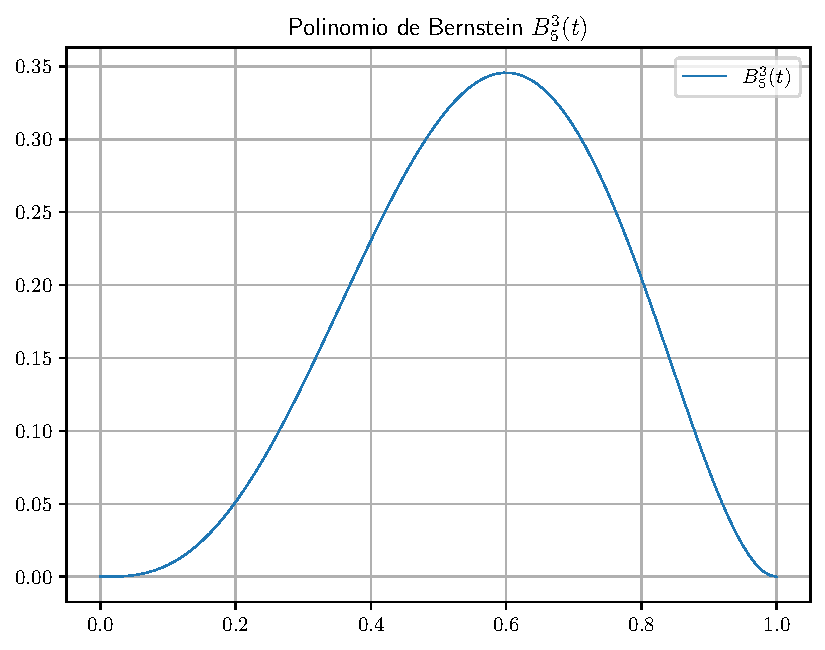
\includegraphics[width=.72\paperwidth]{p1}
        \end{figure}
    \end{solution}
\end{frame}

\begin{frame}
    \begin{solution}
        \begin{figure}[ht!]
            \centering
            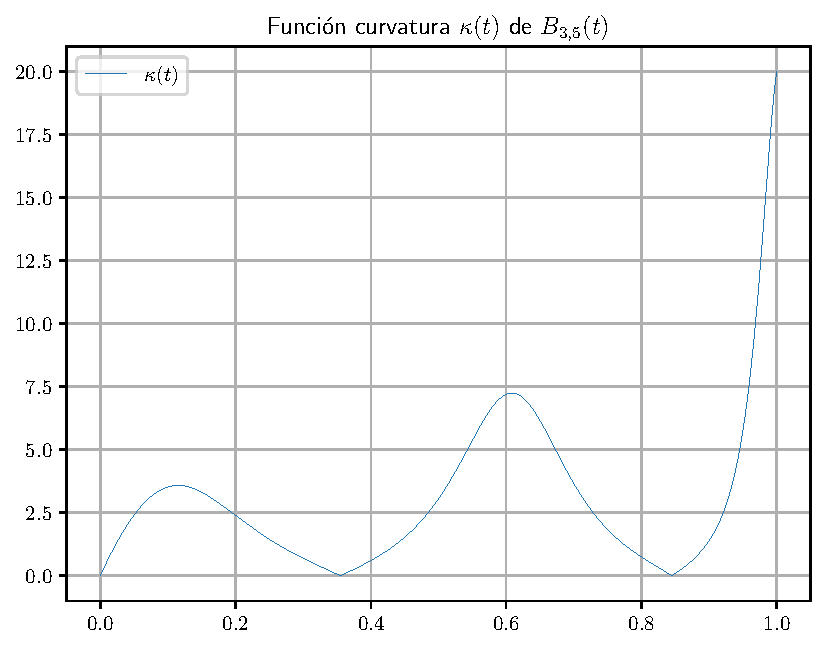
\includegraphics[width=.72\paperwidth]{p1_curvature}
        \end{figure}
    \end{solution}
\end{frame}

\begin{frame}[fragile]
    Las gráficas de los polinomios de Bernstein y su curvatura fueron
    obtenidas del programa en Python.
    \begin{solution}
        \begin{columns}
            \begin{column}{0.48\textwidth}
                \inputminted[fontsize=\tiny,firstline=3,lastline=4]{python}{p1.py}

                \

                \inputminted[fontsize=\tiny,firstline=10,lastline=20]{python}{p1.py}

            \end{column}
            \begin{column}{0.48\textwidth}
                \inputminted[fontsize=\tiny,firstline=23,lastline=27]{python}{p1.py}

                \

                \inputminted[fontsize=\tiny,firstline=34,lastline=40]{python}{p1.py}
            \end{column}
        \end{columns}
    \end{solution}
\end{frame}
\section{Pregunta N$^{\circ}$3\qquad Leon Alonzo Terrones Caccha}

\begin{frame}
    \begin{enumerate}\setcounter{enumi}{2}
        \item
              Demostrar que las funciones de Bernstein para $n=3$ son linealmente independiente.

              \[\sum_{k=0}^{3}=c_{k}B_{k,3}(t)\]

    \end{enumerate}

    \begin{solution}
        Sea la combinación lineal con $c_k\in\mathbb{R}:$
        \[\sum_{k=0}^{3}=c_{k}B_{k,3}(t)\]
        Por demostrar que $c_k=0$, $i\in[0.3]$
        \begin{align*}
            \sum_{k=0}^{3}=c_{k}B_{k,3}(t) & =\sum_{k=0}^{3}c_k\binom{3}{k}t^k(1-t)^{3-k}                                        \\
                                           & =\sum_{k=0}^{3}{c_k\binom{3}{k}t^k\sum_{j=0}^{n-k}\binom{3-k}{j}{(-t)^{3-k-j}}}     \\
                                           & =\sum_{j=0}^{3}{t^{n-j}\sum_{k=0}^{3-j}{c_k\binom{3}{k}\binom{3-k}{j}(-1)^{3-k-j}}}
        \end{align*}

        El cual es un polinomio de gra
        Para $j=0$, el coeficiente de $t^3$ es:
        \begin{align*}
            \sum_{k=0}^{3}{c_k\binom{3}{k}\binom{3-k}{0}(-1)^{3-k}} & =3(-3c_0+3c_1-3c_2+3c_3)
        \end{align*}
    \end{solution}
\end{frame}

\begin{frame}
    \begin{solution}
        Al final se obtiene un sistema lineal en funcion del vector $c=(c_0,c_1,c_2,c_3)$. Debido a que $\{1,t,t^2,t^3\}$ es una base para los polinomios de grado 3 se tiene que $a_k=0$. Finalmente aplicando sustitución progresiva se obtiene $c_k=0$, $k\in[0.3]$.
    \end{solution}
\end{frame}

\section{Pregunta N$^{\circ}$4\qquad Andre Gilmer Santos Felix}

\begin{frame}
	\begin{enumerate}\setcounter{enumi}{3}
		\item

		      Demuestre que
		      \begin{math}
			      \forall n\in\mathbb{N}:
			      B_{n}\left(x\right)=
			      \left(\dfrac{n-1}{n}\right)x^{2}+
			      \dfrac{1}{n}x
		      \end{math}
		      y determine un $n_{0}$ tal que
		      \begin{math}
			      \left|
			      B_{n_{0}}\left(x\right)
			      \right|\leq
			      10^{-6}
		      \end{math}
		      se satisface para todo $x\in\left[0,1\right]$.
	\end{enumerate}

	\begin{solution}
		.
	\end{solution}
\end{frame}

\section{Pregunta N$^{\circ}$6\qquad León Alonzo Terrones Caccha}

\begin{frame}
	\frametitle{Interpolación polinomial}

	\begin{definition}[Conjunto nodal]
		Sea
		\begin{math}
			\left[a,b\right]\subset
			\mathbb{R}
		\end{math}.
		$T$ es un \alert{conjunto nodal} de tamaño
		$n+1\in\mathbb{N}$ en $\left[a,b\right]$ sii
		\begin{math}
			T=
			{
			\left\{
			t_{i}
			\right\}
			}^{n}_{i=0}\subset
			\left[a,b\right]
		\end{math}
		es un conjunto de elementos distintos.
		Los elementos de $T$, $t_{i}$ son llamados \alert{nodos}.
	\end{definition}

	\begin{definition}[Polinomio interpolante]
		Sean
		\begin{math}
			T=
			{
			\left\{
			t_{i}
			\right\}
			}^{n}_{i=0}\subset
			\left[a,b\right]
		\end{math}
		un conjunto nodal y
		\begin{math}
			f\colon
			\left[a,b\right]\to
			\mathbb{R}
		\end{math}
		una función.
		La función $I\colon\left[a,b\right]\to\mathbb{R}$ es llamada un
		\alert{interpolante de} $f$ subordinado a $T$ sii
		\begin{math}
			\forall i\in\left\{0,\dotsc,n\right\}:
			I\left(t_{i}\right)=f\left(t_{i}\right)
		\end{math}.
		En este caso, escribimos
		\begin{math}
			I\left(T\right)=
			f\left(T\right)
		\end{math}.
	\end{definition}

	\begin{definition}[Polinomio de interpolación]
		Sea
		\begin{math}
			X=
			{
			\left\{
			x_{i}
			\right\}
			}^{n}_{i=0}\subset
			\mathbb{R}
		\end{math}
		un conjunto de puntos no necesariamente distintos.
		Defina el conjunto de pares ordenados
		\begin{equation*}
			O\coloneqq
			\left\{
			\left(x_{i},y_{i}\right)\mid
			t_{i}\in T,
			x_{i}\in X,
			\forall i\in\left\{0,\dotsc,n\right\}
			\right\}
		\end{equation*}
		$I$ es un interpolante de $O$ sii
		\begin{math}
			\forall i\in\left\{0,\dotsc,n\right\}:
			I\left(t_{i}\right)=
			f\left(t_{i}\right)
		\end{math},
		es decir, $I\left(T\right)=X$.
		Si el interpolante $I$ es un polinomio, este es llamado un
		\alert{polinomio de interpolación}.
	\end{definition}

	% Sean $n+1$ puntos distintos
	% \begin{math}
	% 	{
	% 		\left\{
	% 		\left(x_{k},y_{k}\right)
	% 		\right\}
	% 	}_{k=0}^{n}\subset
	% 	\left[a,b\right]\times\mathbb{R}
	% \end{math}
	% y
	% \begin{math}
	% 	f\colon\left[a,b\right]\to
	% 	\mathbb{R}
	% \end{math}
	% una función de modo que
	% \begin{math}
	% 	y_{k}=
	% 	f\left(x_{k}\right)
	% \end{math}
	% para $0\leq k\leq n$.

	% Here $\ell_{0},\ell_{1},\ldots,\ell_{n}$ are polynomials that
	% depend on the nodes $x_0, x_1, \ldots, x_n$ but not on the
	% ordinates $y_{0},y_{1},\ldots,y_{n}$.
	% Since all the ordinates could be $0$ except for a $1$ occupying the
	% $i$-th position, we see that

	% \begin{equation*}
	% 	\delta_{ij}=
	% 	p_{n}
	% 	\left(x_j\right)=
	% 	\sum\limits_{k=0}^{n}
	% 	y_{k}
	% 	\ell_k\left(x_j\right)=
	% 	\sum\limits_{k=0}^{n}
	% 	\delta_{ki}
	% 	\ell_{k}
	% 	\left(x_j\right)=
	% 	\ell_{i}
	% 	\left(x_j\right).
	% \end{equation*}

	% (Recall that the Kronecker delta is defined by $\delta_{k i}=1$ if
	% $k=i$ and $\delta_{k i}=0$ if $k \neq i$.)
	% We can easily arrive at a set of polynomials having this property.
	% Let us consider $\ell_{0}$.
	% It is to be a polynomial of degree $n$ that takes the value $0$ at
	% $x_{1},x_{2},\ldots,x_{n}$ and the value $1$ at $x_0$.
	% Clearly, $\ell_{0}$ must be of the form

	% \begin{equation*}
	% 	\ell_{0}
	% 	\left(x\right)=
	% 	c
	% 	\left(x-x_1\right)
	% 	\left(x-x_2\right)\cdots
	% 	\left(x-x_n\right)=
	% 	c
	% 	\prod\limits_{j=1}^{n}
	% 	\left(x-x_j\right).
	% \end{equation*}

	% The value of $c$ is obtained by putting $x=x_{0}$, so that
	% \begin{math}
	% 	1=
	% 	c
	% 	\prod\limits_{j=1}^{n}
	% 	\left(x_{0}-x_{j}\right)
	% \end{math}
	% y
	% \begin{math}
	% 	c=
	% 	\prod\limits_{j=1}^{n}
	% 	{\left(x_{0}-x_{j}\right)}^{-1}
	% \end{math}.

	\begin{definition}[Matriz de Vandermonde]
		Sea
		\begin{math}
			T=
			{
			\left\{
			t_{i}
			\right\}
			}^{n}_{i=0}
		\end{math}
		un conjunto nodal.
		La \alert{matriz de Vandermonde} subordinada al conjunto
		nodal $T$, denotada por
		\begin{math}
			V_{n}=
			\left[v_{ij}\right]\in
			\mathbb{R}^{\left(n+1\right)\times\left(n+1\right)}
		\end{math}
		es la matriz con entradas
		\begin{math}
			\forall\left\{i,j\right\}\subset
			\left\{1,\dotsc,n+1\right\}:
			v_{ij}=
			t^{j-1}_{i-1}
		\end{math},
		es decir,
		\begin{equation*}
			V_{n}=
			\begin{bmatrix}
				1      & t_{0} & \cdots & t_{0}^{n} \\
				\vdots & t_{1} & \ddots & \vdots    \\
				1      & t_{n} & \cdots & t_{n}^{n}
			\end{bmatrix}.
		\end{equation*}
	\end{definition}
\end{frame}

\begin{frame}
	\begin{definition}[Operador de interpolación]
		Sea
		\begin{math}
			T=
			{
			\left\{
			t_{i}
			\right\}
			}^{n}_{i=0}
		\end{math}
		un conjunto nodal.
		El \alert{operador de interpolación} subordinado a $T$ es
		\begin{math}
			\mathcal{I}_{T}:
			C\left(\left[a,b\right]\right)\to
			\mathbb{P}_{n}
		\end{math}
		donde
		\begin{math}
			\mathcal{I}_{T}
			\left[f\right]
		\end{math}
		es el único polinomio de interpolación
		que satisface
		\begin{math}
			\mathcal{I}_{T}
			\left[f\right]
			\left(T\right)=
			f\left(T\right)
		\end{math}.
	\end{definition}

	\begin{theorem}[Operador de proyección lineal]
		Sea
		\begin{math}
			T=
			{
			\left\{
			t_{i}
			\right\}
			}^{n}_{i=0}
			\subset\left[a,b\right]
		\end{math}
		un conjunto nodal e
		\begin{math}
			\mathcal{I}_{T}:
			C\left(\left[a,b\right]\right)\to
			\mathbb{P}_{n}
		\end{math}
		es el operador de interpolación subordinado a $T$.
		\begin{math}
			\mathcal{I}_{T}
		\end{math}
		es un \alert{operador de proyección lineal} sii
		\begin{equation*}
			\forall f,g\in C\left(\left[a,b\right]\right):
			\forall\alpha\in\mathbb{R}:
			\mathcal{I}_{T}\left[\alpha f+g\right]=
			\alpha\mathcal{I}_{T}\left[f\right]+
			\mathcal{I}_{T}\left[g\right],\qquad
			\forall p\in\mathbb{P}_{n}:
			\mathcal{I}_{T}\left[p\right]=
			p.
		\end{equation*}
	\end{theorem}

	\begin{definition}[Constante de Lebesgue]
		Sea
		\begin{math}
			T=
			{
			\left\{
			t_{i}
			\right\}
			}^{n}_{i=0}
			\subset\left[a,b\right]
		\end{math}
		un conjunto nodal e
		\begin{math}
			\mathcal{I}_{T}:
			C\left(\left[a,b\right]\right)\to
			\mathbb{P}_{n}
		\end{math}
		es el operador de interpolación subordinado a $T$.
		La \alert{constante de Lebesgue subordinada a} $T$,
		$\Lambda\left(T\right)$, es la norma del operador
		$\mathcal{I}_{T}$, es
		decir,
		\begin{math}
			\Lambda\left(T\right)=
			{\left\|
			\mathcal{I}_{T}
			\right\|}_{\infty}
		\end{math},
		donde
		\begin{equation*}
			{\left\|
				\mathcal{I}_{T}
				\right\|}_{\infty}=
			\sup_{f\neq0}
			\dfrac{
				{\left\|
						\mathcal{I}_{T}
						\left[f\right]
						\right\|}_{\infty}
			}{
				{\left\|f\right\|}_{\infty}
			}=
			\sup_{
				{\left\|f\right\|}_{\infty}=1}
			\left\|
			\mathcal{I}_{T}
			\left[f\right]
			\right\|_{\infty}.
		\end{equation*}
	\end{definition}
\end{frame}

\begin{frame}
	\begin{definition}[Polinomio de interpolación en la forma de Lagrange]
		Sea
		\begin{math}
			T=
			{
			\left\{
			t_{i}
			\right\}
			}^{n}_{i=0}
			\subset\left[a,b\right]
		\end{math}
		un conjunto nodal.
		El \alert{polinomio de interpolación de Lagrange} de la función $f$,
		subordinada al conjunto nodal $T$, es el polinomio
		\begin{equation*}
			\Pi_{n}
			f\left(t\right)\coloneqq
			% y_{0}
			% \ell_{0}\left(x\right)+
			% y_{1}
			% \ell_{1}\left(x\right)+
			% \cdots+
			% y_{n}
			% \ell_{n}\left(x\right)=
			\sum\limits_{k=0}^{n}
			x_{k}
			\ell_{k}\left(t\right)\in\mathbb{P}_{n},
		\end{equation*}
		donde
		\begin{math}
			\ell_{k}
			\left(t\right)\coloneqq
			\prod\limits_{\substack{j=0\\j\neq k}}^{n}
			\dfrac{t-t_{j}}{t_{k}-t_{j}}
		\end{math}
		para $0\leq k\leq n$ son las \alert{bases nodales de Lagrange}
		que satisface
		\begin{math}
			\ell_{k}
			\left(t_{j}\right)=
			\delta_{kj}
		\end{math}.

		La evaluación de $\Pi_{n}f\left(t\right)$ requiere
		$O\left(n^{2}\right)$ sumas y productos, en general el
		algoritmo es \emph{numéricamente inestable}.
	\end{definition}

	\begin{definition}[Polinomio de interpolación en la forma de Newton]
		\begin{equation*}
			\Pi_{n}
			f\left(t\right)\coloneqq
			\sum\limits_{k=0}^{n}
			a_{k}
			\omega_{k}\left(t\right)\in\mathbb{P}_{n},
		\end{equation*}
		donde
		\begin{itemize}
			\item

			      \begin{math}
				      a_{k}\coloneqq
				      f\left[t_{0},\ldots,t_{k}\right]
			      \end{math}
			      es la \alert{$k$-ésima diferencia dividida de Newton}, y

			\item

			      \begin{math}
				      \omega_{k}
				      \left(t\right)\coloneqq
				      \prod\limits_{j=0}^{k-1}
				      \left(
				      t-t_{j}
				      \right)
			      \end{math}
			      es el \alert{polinomio nodal de grado $k$}.
		\end{itemize}
		La evaluación de $\Pi_{n}f\left(t\right)$ requiere
		$O\left(n\right)$.
	\end{definition}
\end{frame}

% https://people.maths.ox.ac.uk/trefethen/barycentric.pdf
% \begin{frame}
% 	\begin{definition}[Interpolación baricéntrica de Lagrange]
% 		Con el fin de realizar menos operaciones en la interpolación
% 		polinomial de Lagrange, multiplicamos por
% 		\begin{math}
% 			\alert{
% 				\dfrac{1}{\omega_{n+1}\left(x\right)}
% 			}
% 		\end{math}
% 		y resulta
% 		\begin{align*}
% 			\alert{
% 				\dfrac{1}{\omega_{n+1}\left(x\right)}
% 			}
% 			\Pi_{n}f\left(x\right) & =
% 			\alert{
% 				\dfrac{1}{\omega_{n+1}\left(x\right)}
% 			}
% 			\sum\limits_{k=0}^{n}
% 			y_{k}
% 			\alert{
% 				\ell_{k}\left(x\right)
% 			}=
% 			\dfrac{1}{\omega_{n+1}\left(x\right)}
% 			\sum\limits_{k=0}^{n}
% 			y_{k}
% 			\alert{
% 			\prod\limits_{\substack{j=0 \\j\neq k}}^{n}
% 			\dfrac{x-x_{j}}{x_{k}-x_{j}}
% 			}.
% 			\\
% 			                       & =
% 			\sum\limits_{k=0}^{n}
% 			\left\{
% 			\dfrac{y_{k}}{
% 				\alert{
% 			\prod\limits_{\substack{j=0 \\j\neq k}}^{n}
% 					\left(
% 					x_{k}-x_{j}
% 					\right)
% 				}
% 			}
% 			\dfrac{
% 				\alert{
% 			\prod\limits_{\substack{j=0 \\j\neq k}}^{n}
% 					\left(
% 					x-x_{j}
% 					\right)
% 				}
% 			}{\omega_{n+1}\left(x\right)}
% 			\right\}=
% 			\sum\limits_{k=0}^{n}
% 			\left\{
% 			\dfrac{y_{k}}{
% 			\prod\limits_{\substack{j=0 \\j\neq k}}^{n}
% 				\left(
% 				x_{k}-x_{j}
% 				\right)
% 			}
% 			\dfrac{1}{x-x_{k}}
% 			\right\}.
% 			\\
% 			\Pi_{n}f\left(x\right)
% 			                       & =
% 			\sum\limits_{k=0}^{n}
% 			y_{k}
% 			\widetilde{\ell}_{k}\left(x\right)\in\mathbb{P}_{n},
% 		\end{align*}
% 		donde
% 		\begin{columns}
% 			\begin{column}{.45\paperwidth}
% 				\begin{itemize}
% 					\item

% 					      \begin{math}
% 						      \widetilde{\ell}_{k}
% 						      \left(x\right)=
% 						      \omega_{n+1}
% 						      \left(x\right)
% 						      \dfrac{b_{k}}{x-x_{k}}
% 					      \end{math}, y
% 				\end{itemize}
% 			\end{column}
% 			\begin{column}{.45\paperwidth}
% 				\begin{itemize}
% 					\item

% 					      \begin{math}
% 						      b_{j}=
% 						      \dfrac{1}{
% 							      \prod\limits_{\substack{j=0\\j\neq k}}^{n}
% 							      \left(
% 							      x_{k}-x_{j}
% 							      \right)
% 						      }
% 					      \end{math}
% 					      son los \emph{pesos baricéntricos}.
% 				\end{itemize}
% 			\end{column}
% 		\end{columns}
% 		% La evaluación de $\Pi_{n}f\left(x\right)$ requiere
% 		% $O\left(n\right)$.
% 	\end{definition}
% \end{frame}
% \begin{frame}
	\begin{theorem}
		Para $0\leq k\leq n$ se cumple
		\begin{math}
			\omega^{\prime}_{n+1}
			\left(x_{k}\right)=
			\prod\limits_{\substack{j=0\\j\neq k}}^{n}
			\left(
			x_{k}-x_{j}
			\right).
		\end{math}
	\end{theorem}

	\begin{proof}
		Si
		\begin{math}
			\omega_{\alert{n+1}}
			\left(x\right)
			\overset{\text{def}}{=}
			\prod\limits_{j=0}^{\alert{n+1}-1}
			\left(
			x-x_{j}
			\right)=
			\prod\limits_{j=0}^{n}
			\left(
			x-x_{j}
			\right)
		\end{math}, entonces
		\begin{math}
			\ln
			\left(
			\omega_{n+1}
			\left(x\right)
			\right)=
			\ln
			\left(
			\prod\limits_{j=0}^{n}
			\left(
				x-x_{j}
				\right)
			\right)=
			\sum\limits_{j=0}^{n}
			\ln
			\left(
			x-x_{j}
			\right)
		\end{math}.
		Derivando,

		\begin{align*}
			{\left(
				\ln
				\left(
					\omega_{n+1}
					\left(x\right)
					\right)
			\right)}^{\prime} & =
			{\left(
			\sum\limits_{j=0}^{n}
			\ln
			\left(
				x-x_{j}
				\right)
			\right)}^{\prime}=
			\sum\limits_{j=0}^{n}
			{\left(
			\ln
			\left(
				x-x_{j}
				\right)
			\right)}^{\prime}.
			\\
			\dfrac{
				\omega^{\prime}_{n+1}\left(x\right)
			}{
				\alert{
					\omega_{n+1}\left(x\right)
				}
			}                 & =
			\sum\limits_{j=0}^{n}
			\dfrac{{\left(x-x_{j}\right)}^{\prime}}{x-x_{j}}=
			\sum\limits_{j=0}^{n}
			\dfrac{1}{x-x_{j}}.
			\\
			\Aboxed{
			w^{\prime}_{n+1}
			\left(x\right)    & =
			\alert{
				\omega_{n+1}
				\left(x\right)
			}
			\sum\limits_{j=0}^{n}
			\dfrac{1}{x-x_{j}}.
			}
			\\
			w^{\prime}_{n+1}
			\left(x_{k}\right)
			                  & =
			\alert{
				\prod\limits_{j=0}^{n}
				\left(
				x_{k}-x_{j}
				\right)
			}
			\sum\limits_{i=0}^{n}
			\dfrac{1}{x_{k}-x_{i}}=
			\prod\limits_{j=0}^{n}
			\sum\limits_{i=0}^{n}
			\dfrac{
			x_{k}-x_{j}
			}{
			x_{k}-x_{i}
			}
			=
			\prod\limits_{\substack{j=0 \\j\neq k}}^{n}
			\left(
			x_{k}-x_{j}
			\right).
		\end{align*}
		% Si $x_{k}$ un punto nodal cualesquiera, donde $0\leq k\leq n$,
		% entonces
		% \begin{math}
		% 	w^{\prime}_{n+1}
		% 	\left(x_{k}\right)=
		% 	\prod\limits_{\substack{j=0 \\j\neq k}}^{n}
		% 	\left(
		% 	x_{k}-x_{j}
		% 	\right)
		% \end{math}.
	\end{proof}
\end{frame}

\begin{frame}
	\begin{theorem}
		Si $\Pi_{n}f\left(x\right)$ es el polinomio de Lagrange, entonces
		\begin{math}
			\Pi_{n}f\left(x\right)=
			\sum\limits_{k=0}^{n}
			\dfrac{
				\omega_{n+1}\left(x\right)
			}{
				\left(x-x_{k}\right)
				\omega^{\prime}_{n+1}\left(x_{k}\right)
			}
			y_{k}
		\end{math}.
	\end{theorem}

	\begin{proof}
		\begin{align*}
			\sum\limits_{k=0}^{n}
			\dfrac{
				\omega_{n+1}\left(x\right)
			}{
				\left(x-x_{k}\right)
				\alert{
					\omega^{\prime}_{n+1}\left(x_{k}\right)
				}
			}
			y_{k} & =
			\sum\limits_{k=0}^{n}
			y_{k}
			\dfrac{
				\prod\limits_{j=0}^{n}
				\left(
				x-x_{j}
				\right)
			}{
				\left(x-x_{k}\right)
				\alert{
			\prod\limits_{\substack{j=0 \\j\neq k}}^{n}
					\left(
					x_{k}-x_{j}
					\right)
				}
			}
			\\
			      & =
			\sum\limits_{k=0}^{n}
			y_{k}
			\dfrac{
			\prod\limits_{\substack{j=0 \\j\neq k}}^{n}
				\left(
				x-x_{j}
				\right)
			}{
			\prod\limits_{\substack{j=0 \\j\neq k}}^{n}
				\left(
				x_{k}-x_{j}
				\right)
			}
			\\
			      & =
			\sum\limits_{k=0}^{n}
			y_{k}
			\alert{
			\prod\limits_{\substack{j=0 \\j\neq k}}^{n}
			\dfrac{
			x-x_{j}
			}{
			x_{k}-x_{j}
			}
			}                           \\
			      & =
			\sum\limits_{k=0}^{n}
			y_{k}
			\alert{
				\ell_{k}\left(x\right)
			}
			=
			\Pi_{n}
			f\left(x\right).
		\end{align*}
	\end{proof}
\end{frame}

\begin{frame}
	\begin{theorem}[Teorema de las diferencias divididas de orden superior]
		Para $0\leq k\leq n$ se cumple
		\begin{equation*}
			a_{k}=
			f\left[x_{0},\ldots,x_{k}\right]=
			\dfrac{
			f\left[x_{1},\ldots,x_{k}\right]-
			f\left[x_{0},\ldots,x_{k-1}\right]
			}{x_{k}-x_{0}}.
			% \begin{cases}
			% 	0 & \text{si} \\
			% 	1 & \text{no}
			% \end{cases}
		\end{equation*}
		La evaluación de $a_{n}$ requiere $n^{2}$ restas y
		$\dfrac{n^{2}}{2}$ divisiones.
	\end{theorem}

	% \begin{proof}
	% 	.
	% \end{proof}

	\begin{theorem}[Representación explícita de $a_{n}$]
		¿Encontrar alguna identidad entre $\omega_{k}\left(x\right)$ y
		$\ell_{k}\left(x\right)$?
		\begin{equation*}
			a_{n}=
			\sum\limits_{k=0}^{n}
			\dfrac{
				f\left(x_{k}\right)
			}{
				w^{\prime}_{n+1}
				\left(x_{k}\right)
			}.
		\end{equation*}
	\end{theorem}

	\begin{proof}
		\begin{equation*}
			\sum\limits_{k=0}^{n}
			\dfrac{
				f\left(x_{k}\right)
			}{
				\alert{
					w^{\prime}_{n+1}
					\left(x_{k}\right)
				}
			}=
			\sum\limits_{k=0}^{n}
			\dfrac{
				f\left(x_{k}\right)
			}{
				\alert{
					\prod\limits_{\substack{j=0 \\j\neq k}}^{n}
					\left(
					x_{k}-x_{j}
					\right)
				}
			}
		\end{equation*}
	\end{proof}

	% \begin{theorem}[Interpolación de Lagrange baricéntrica] % Fórmula baricéntrica
	% 	\begin{equation*}
	% 		\lambda_{k}\coloneqq
	% 		\prod\limits_{\substack{j=0               \\j\neq k}}^{n}
	% 		\dfrac{1}{x_{k}-x_{j}}=
	% 		\dfrac{1}{\prod\limits_{\substack{j=0               \\j\neq k}}^{n}x_{k}-x_{j}}
	% 	\end{equation*}
	% \end{theorem}
\end{frame}

\begin{frame}
	\begin{enumerate}\setcounter{enumi}{5}
		\item

		      Encuentre el interpolante de Lagrange
		      \begin{math}
			      p_{2}\left(t\right)=
			      \sum\limits_{k=0}^{2}
			      x_{k}
			      \ell_{k}\left(t\right)
		      \end{math}
		      para el conjunto de datos
		      \begin{math}
			      \left\{
			      \left(0,1\right),
			      \left(\frac{1}{2},2\right),
			      \left((1,\frac{3}{2}\right),
                    \left((2,-1\right)
			      \right\}
		      \end{math}.
		      Encuentre $p_{2,k}$ en
		      \begin{math}
			      p_{2}\left(t\right)=
			      \sum\limits_{k=0}^{2}
			      p_{2,k}t^{k}
		      \end{math}.
	\end{enumerate}

	\begin{solution}
		\begin{align*}
			\ell_{0}\left(t\right) & =
			\prod\limits_{\substack{j=0        \\j\neq 0}}^{n}
			\dfrac{t-t_{j}}{t_{0}-t_{j}}=
			\dfrac{\left(t-t_{1}\right)\left(t-t_{2}\right)}{\left(t_{0}-t_{1}\right)\left(t_{0}-t_{2}\right)}=
			\dfrac{\left(t-0\right)\left(t-1\right)}{\left(\left(-1\right)-0\right)\left(\left(-1\right)-1\right)}=
			\dfrac{1}{2}t\left(t-1\right).     \\
			\ell_{1}\left(t\right) & =
			\prod\limits_{\substack{j=0        \\j\neq 1}}^{n}
			\dfrac{t-t_{j}}{t_{1}-t_{j}}=
			\dfrac{\left(t-t_{0}\right)\left(t-t_{2}\right)}{\left(t_{1}-t_{0}\right)\left(t_{1}-t_{2}\right)}=
			\dfrac{\left(t-\left(-1\right)\right)\left(t-1\right)}{\left(0-\left(-1\right)\right)\left(0-1\right)}=
			-\left(t+1\right)\left(t-1\right). \\
			\ell_{2}\left(t\right) & =
			\prod\limits_{\substack{j=0        \\j\neq 2}}^{n}
			\dfrac{t-t_{j}}{t_{2}-t_{j}}=
			\dfrac{\left(t-t_{0}\right)\left(t-t_{1}\right)}{\left(t_{2}-t_{0}\right)\left(t_{2}-t_{1}\right)}=
			\dfrac{\left(t-\left(-1\right)\right)\left(t-0\right)}{\left(1-\left(-1\right)\right)\left(1-0\right)}=
			\dfrac{1}{2}\left(t+1\right)t.
		\end{align*}

		Entonces,
		\begin{align*}
			p_{2}\left(t\right) & =
			\sum\limits_{k=0}^{2}
			x_{k}
			\ell_{k}\left(t\right)=
			\alert{x_{0}}\ell_{0}\left(t\right)+
			\alert{x_{1}}\ell_{1}\left(t\right)+
			\alert{x_{2}}\ell_{2}\left(t\right)=
			\dfrac{1}{2}\ell_{0}\left(t\right)+
			\ell_{1}\left(t\right)-
			\ell_{2}\left(t\right).               \\
			                    & =
			\dfrac{1}{2}\alert{\dfrac{1}{2}t\left(t-1\right)}
			\alert{-\left(t+1\right)\left(t-1\right)}-
			\alert{\dfrac{1}{2}\left(t+1\right)t}. \\
			                    & =
			-1.25t^{2}-0.75t+1.
		\end{align*}
	\end{solution}
\end{frame}

\begin{frame}
	\begin{solution}
		\begin{figure}[ht!]
			\centering
			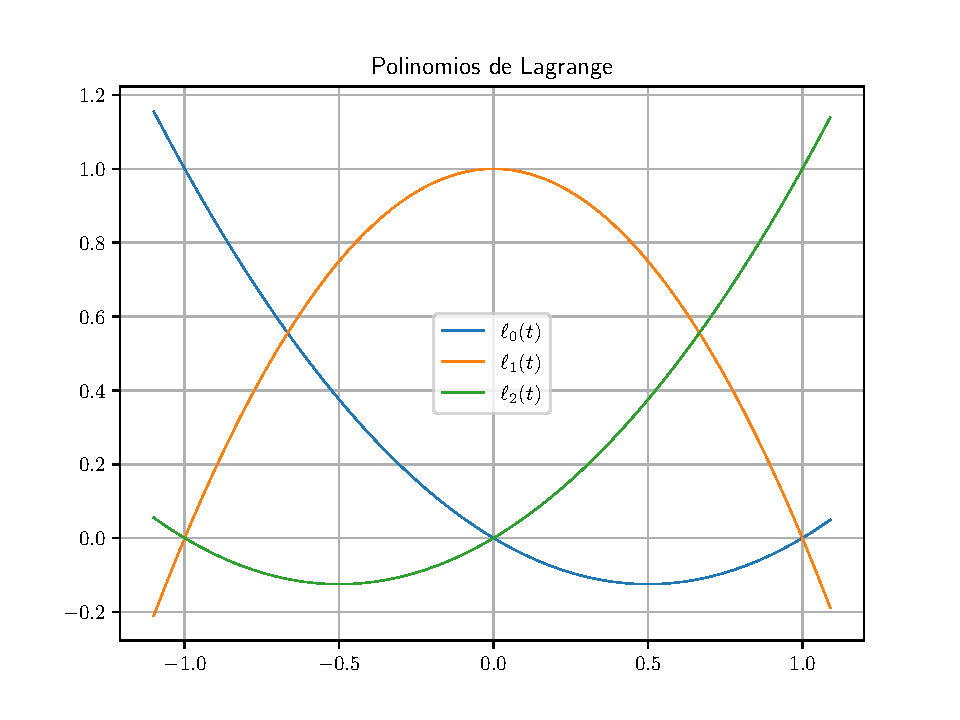
\includegraphics[width=.8\paperwidth]{p6_lagrange}
		\end{figure}
	\end{solution}
\end{frame}


\begin{frame}
	\begin{solution}
		\begin{figure}[ht!]
			\centering
			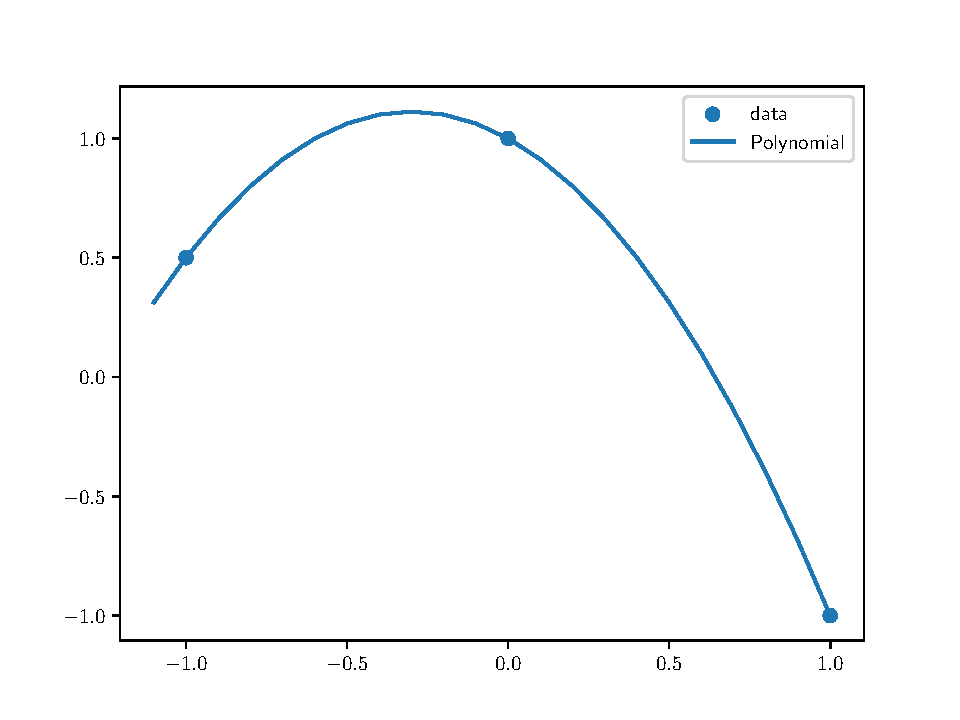
\includegraphics[width=.8\paperwidth]{p6}
		\end{figure}
	\end{solution}
\end{frame}
\section{Pregunta N$^{\circ}$7\qquad Andre Gilmer Santos Felix}

\begin{frame}
	\begin{enumerate}\setcounter{enumi}{6}
		\item

		      Encuentre el interpolante de Lagrange
		      \begin{math}
			      p_{3}\left(t\right)=
			      \sum\limits_{k=0}^{3}
			      x_{k}
			      \ell_{k}\left(t\right)
		      \end{math}
		      para el conjunto de datos
		      \begin{math}
			      \left\{
			      \left(0,1\right),
			      \left(\frac{1}{2},2\right),
			      \left((1,\frac{3}{2}\right),
			      \left((2,-1\right)
			      \right\}
		      \end{math}.
		      Encuentre $p_{2,k}$ en
		      \begin{math}
			      p_{3}\left(t\right)=
			      \sum\limits_{k=0}^{3}
			      p_{3,k}t^{k}
		      \end{math}.
	\end{enumerate}

	\begin{solution}
		\begin{align*}
			\ell_{0}\left(t\right) & =
			\prod\limits_{\substack{j=0 \\j\neq 0}}^{n}
			\dfrac{t-t_{j}}{t_{0}-t_{j}}=
			\dfrac{\left(t-t_{1}\right)\left(t-t_{2}\right)\left(t-t_{3}\right)}{\left(t_{0}-t_{1}\right)\left(t_{0}-t_{2}\right)\left(t_{0}-t_{3}\right)}=
			\dfrac{\left(t-\dfrac{1}{2}\right)\left(t-1\right)\left(t-2\right)}{\left(0-\dfrac{1}{2}\right)\left(0-1\right)\left(0-2\right)}=
			0.                          \\
			\ell_{1}\left(t\right) & =
			\prod\limits_{\substack{j=0 \\j\neq 1}}^{n}
			\dfrac{t-t_{j}}{t_{1}-t_{j}}=
			\dfrac{\left(t-t_{0}\right)\left(t-t_{2}\right)\left(t-t_{3}\right)}{\left(t_{1}-t_{0}\right)\left(t_{1}-t_{2}\right)\left(t_{1}-t_{3}\right)}=
			\dfrac{\left(t-0\right)\left(t-1\right)\left(t-2\right)}{\left(\dfrac{1}{2}-0\right)\left(\dfrac{1}{2}-1\right)\left(\dfrac{1}{2}-2\right)}=
			0.                          \\
			\ell_{2}\left(t\right) & =
			\prod\limits_{\substack{j=0 \\j\neq 2}}^{n}
			\dfrac{t-t_{j}}{t_{2}-t_{j}}=
			\dfrac{\left(t-t_{0}\right)\left(t-t_{1}\right)\left(t-t_{3}\right)}{\left(t_{2}-t_{0}\right)\left(t_{2}-t_{1}\right)\left(t_{2}-t_{3}\right)}=
			\dfrac{\left(t-0\right)\left(t-\dfrac{1}{2}\right)\left(t-2\right)}{\left(1-0\right)\left(1-\dfrac{1}{2}\right)\left(1-2\right)}=
			0.                          \\
			\ell_{3}\left(t\right) & =
			\prod\limits_{\substack{j=0 \\j\neq 3}}^{n}
			\dfrac{t-t_{j}}{t_{3}-t_{j}}=
			\dfrac{\left(t-t_{0}\right)\left(t-t_{1}\right)\left(t-t_{2}\right)}{\left(t_{3}-t_{0}\right)\left(t_{3}-t_{1}\right)\left(t_{3}-t_{2}\right)}=
			\dfrac{\left(t-0\right)\left(t-\dfrac{1}{2}\right)\left(t-1\right)}{\left(2-0\right)\left(2-\dfrac{1}{2}\right)\left(2-1\right)}=
			0.
			\shortintertext{Entonces,}
			p_{3}\left(t\right)    & =
			\sum\limits_{k=0}^{3}
			x_{k}
			\ell_{k}\left(t\right)=
			\alert{x_{0}}\ell_{0}\left(t\right)+
			\alert{x_{1}}\ell_{1}\left(t\right)+
			\alert{x_{2}}\ell_{2}\left(t\right)+
			\alert{x_{3}}\ell_{3}\left(t\right)=
			\ell_{0}\left(t\right)+
			2\ell_{1}\left(t\right)-
			\dfrac{3}{2}\ell_{2}\left(t\right)-
			\ell_{3}\left(t\right).     \\
			                       & =
			\alert{0}+
			2\alert{0}-
			\dfrac{3}{2}\alert{0}-
			\alert{0}=
			0.
		\end{align*}
	\end{solution}
\end{frame}

% \begin{frame}
% 	\begin{solution}
% 		\begin{figure}[ht!]
% 			\centering
% 			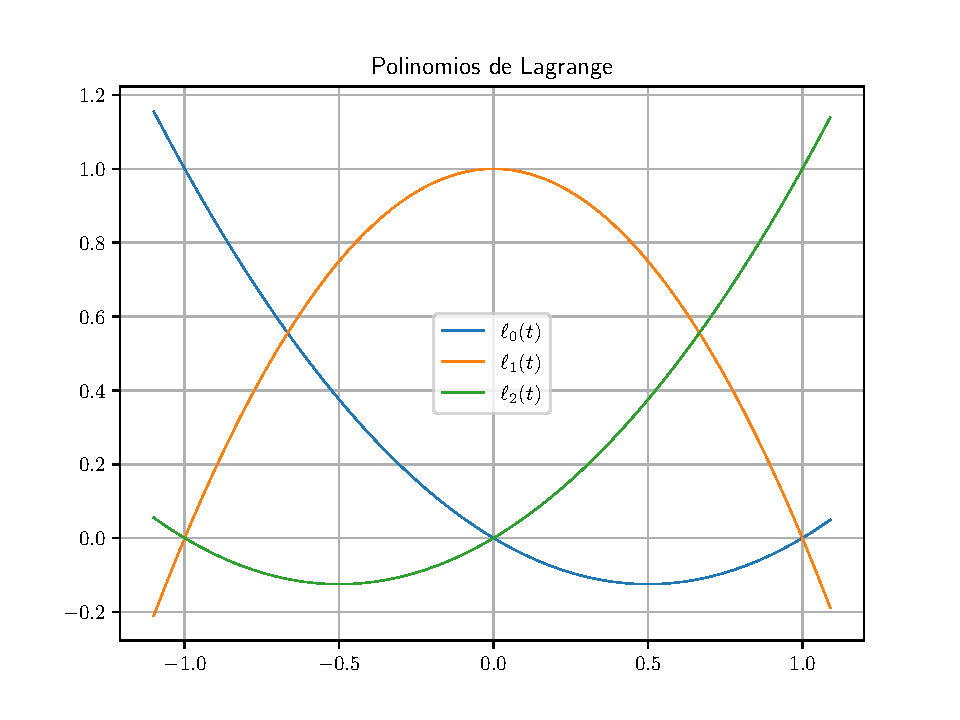
\includegraphics[width=.8\paperwidth]{p6_lagrange}
% 		\end{figure}
% 	\end{solution}
% \end{frame}

\begin{frame}
	\begin{solution}
		\begin{figure}[ht!]
			\centering
			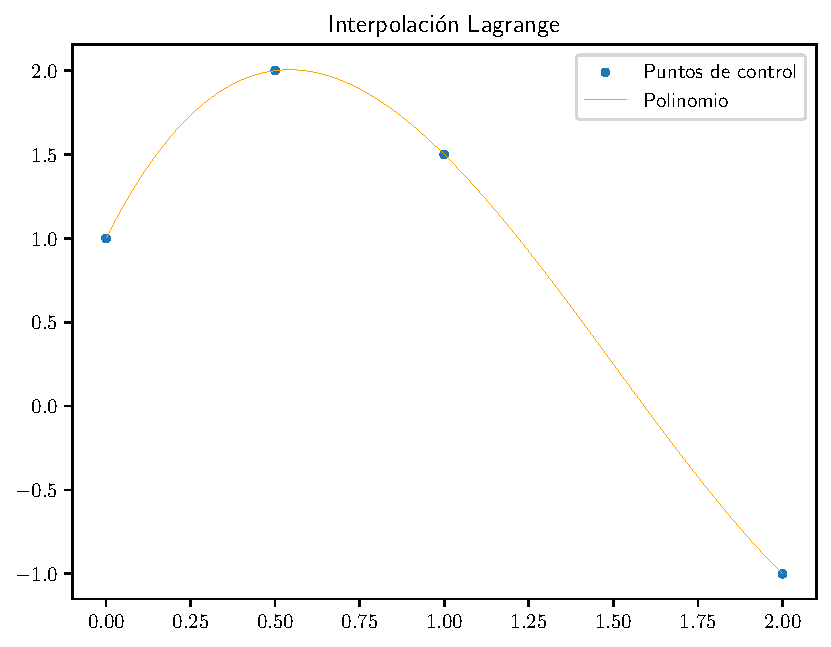
\includegraphics[width=.8\paperwidth]{p7}
		\end{figure}
	\end{solution}
\end{frame}
\section{Pregunta N$^{\circ}$9\qquad Carlos Alonso Aznarán Laos}

\begin{frame}
    \begin{enumerate}\setcounter{enumi}{8}
        \item

              Encuentre una expresión general para
              \begin{math}
                  L_{j}^{\left(1\right)}\left(t\right)=
                  \diff{L_{j}\left(t\right)}{t}
              \end{math}.
    \end{enumerate}

    \begin{solution}
        Vea el teorema de la página 10.
    \end{solution}
\end{frame}
\section{Pregunta N$^{\circ}$11\qquad Leon Alonzo Terrones Caccha}

\begin{frame}
	\begin{theorem}[El Principio de Inducción Matemática]
		Sea $F$ un \alert{cuerpo ordenado}.
		Suponga que $\forall n\in\mathbb{N}_{F}$, $p\left(n\right)$ es
		una proposición acerca de $n$.
		Si

		\begin{multicols}{2}
			\begin{enumerate}[(1)]
				\item\label{hyp:1}

				$p\left(1\right)$ es verdadero, y

				\item\label{hyp:2}

				$\forall k\in\mathbb{N}_{F}$,
				$p\left(k\right)\implies p\left(k+1\right)$,
			\end{enumerate}
		\end{multicols}

		entonces $\forall n\in\mathbb{N}_{F}$, $p\left(n\right)$ es
		verdadero.
	\end{theorem}

	\begin{proof}
		Suponga que $p\left(n\right)$ es como se describe en la
		hipótesis.
		Sea
		\begin{math}
			A=
			\left\{
			x\in\mathbb{N}_{F}:
			p\left(x\right)\text{ es verdadero}
			\right\}
		\end{math}.
		Entonces,
		\begin{enumerate}[(i)]
			\item

			      $1\in A$, por~\eqref{hyp:1}.

			\item

			      Suponga que $x\in A$. Entonces, $x\in\mathbb{N}_{F}$ y
			      $p\left(x\right)$ es verdadero.
			      Así, por~\eqref{hyp:2}, $p\left(x+1\right)$ es verdadero.
			      Esto es, $x+1\in A$.
			      Por lo tanto, $x\in A\implies x+1\in A$.
			      Finalmente, $A$ es conjunto inductivo y
			      $\mathbb{N}_{F}\subset A$.
			      Esto es, $\forall n\in\mathbb{N}_{F}$, $p\left(n\right)$
			      es verdadero.
		\end{enumerate}
	\end{proof}
\end{frame}

\begin{frame}
	\begin{enumerate}\setcounter{enumi}{10}
		\item

		      Pruebe que el
		      \begin{math}
			      \begin{vmatrix}
				      A_{n}
			      \end{vmatrix}=
			      \prod\limits_{\mathclap{0\leq i< j\leq n}}
			      \left(t_{j}-t_{i}\right)
		      \end{math},
		      donde
		      \begin{math}
			      A_{n}=
			      \begin{bmatrix}
				      1      & \cdots & t_{0}^{n} \\
				      \vdots & \ddots & \vdots    \\
				      1      & \cdots & t_{n}^{n}
			      \end{bmatrix}
		      \end{math}
		      es la matriz de Vandermonde.
	\end{enumerate}

	\begin{solution}
		Sean $n\in\mathbb{N}$ y
		\begin{math}
			p\left(n\right)\coloneqq
			\left|A_{n}\right|=
			\prod\limits_{\mathclap{0\leq i< j\leq n}}
			\left(t_{j}-t_{i}\right)
		\end{math}.
		Por el \alert{Principio de Inducción Matemática} sobre $n$,

		\begin{itemize}
			\item

			      \begin{math}
				      p\left(1\right)=
				      \begin{vmatrix}
					      A_{1}
				      \end{vmatrix}=
				      \begin{vmatrix}
					      1 & t_{0} \\
					      1 & t_{1}
				      \end{vmatrix}=
				      t_{1}-t_{0}=
				      \prod\limits_{\mathclap{0\leq i< j\leq 1}}
				      t_{j}-t_{i}
			      \end{math}
			      es verdadero.

			\item

			      Supongamos que $p\left(k\right)$ es verdadero,
			      es decir,
			      \begin{math}
				      \left|
				      A_{k}
				      \right|=
				      \prod\limits_{\mathclap{0\leq i< j\leq k}}
				      \left(t_{j}-t_{i}\right)=
				      \begin{vmatrix}
					      1      & \cdots & t_{0}^{k} \\
					      \vdots & \ddots & \vdots    \\
					      1      & \cdots & t_{k}^{k}
				      \end{vmatrix}.
			      \end{math}
			      Veamos que $p\left(k+1\right)$ es verdadero.

			      \begin{align*}
				      \left|
				      A_{k+1}
				      \right| & =
				      \begin{vmatrix}
					      1      & t_{0}   & \cdots & t_{0}^{k+1}   \\
					      1      & t_{1}   & \cdots & t_{1}^{k+1}   \\
					      \vdots & \vdots  & \ddots & \vdots        \\
					      1      & t_{k+1} & \cdots & t_{k+1}^{k+1}
				      \end{vmatrix}
				      \overset{\left(\star\right)}{=}
				      \begin{vmatrix}
					      1      & t_{0}-\alert{1}\cdot t_{0}   & \cdots & t_{0}^{k+1}-\alert{t_{0}^{k}}\cdot t_{0}     \\
					      1      & t_{1}-\alert{1}\cdot t_{0}   & \cdots & t_{1}^{k+1}-\alert{t_{1}^{k}}\cdot t_{0}     \\
					      \vdots & \vdots                       & \ddots & \vdots                                       \\
					      1      & t_{k+1}-\alert{1}\cdot t_{0} & \cdots & t_{k+1}^{k+1}-\alert{t_{k+1}^{k}}\cdot t_{0}
				      \end{vmatrix}=
				      \begin{vmatrix}
					      1      & 0             & \cdots & 0                                   \\
					      1      & t_{1}-t_{0}   & \cdots & \left(t_{1}-t_{0}\right)t_{1}^{k}   \\
					      \vdots & \vdots        & \ddots & \vdots                              \\
					      1      & t_{k+1}-t_{0} & \cdots & \left(t_{k+1}-t_{0}\right)t_{k}^{k}
				      \end{vmatrix}. \\
				              & =
				      \begin{vmatrix}
					      t_{1}-t_{0}   & \cdots & \left(t_{1}-t_{0}\right)t_{1}^{k}   \\
					      \vdots        & \ddots & \vdots                              \\
					      t_{k+1}-t_{0} & \cdots & \left(t_{k+1}-t_{0}\right)t_{k}^{k}
				      \end{vmatrix}=
				      \prod\limits_{\mathclap{0 <j\leq k+1}}
				      \left(t_{j}-t_{0}\right)
				      \alert{
					      \begin{vmatrix}
						      1      & \cdots & t_{1}^{k} \\
						      \vdots & \ddots & \vdots    \\
						      1      & \cdots & t_{k}^{k}
					      \end{vmatrix}
				      }\overset{\text{H.I.}}{=}
				      \prod\limits_{\mathclap{0 <j\leq k+1}}
				      \left(t_{j}-t_{0}\right)
				      \alert{
					      \prod\limits_{\mathclap{0\leq i< j\leq k}}
					      \left(t_{j}-t_{i}\right)
				      }
				      =
				      \prod\limits_{\mathclap{0\leq i< j\leq k+1}}
				      \left(t_{j}-t_{i}\right).
			      \end{align*}
			      En $\left(\star\right)$, hemos aplicado las operaciones
			      \begin{math}
				      \forall j\in\left\{2,\dotsc,k+1\right\}:
				      c_{j+1}\leftarrow
				      c_{j+1}-c_{j}\cdot t_{0}
			      \end{math}.
			      $\therefore\forall n\in\mathbb{N}$, $p\left(n\right)$ es
			      verdadero.
			      % $A_{n}$ la matriz de Vandermonde asociada al sistema
			      % que halla los coeficientes del polinomio de interpolación
			      % para $n+1$ puntos distintos.
		\end{itemize}
	\end{solution}
\end{frame}
\section{Pregunta N$^{\circ}$12\qquad Carlos Alonso Aznarán Laos}

\begin{frame}
    \begin{enumerate}\setcounter{enumi}{11}
        \item

              Sea
              \begin{math}
                  f\left(t\right)=
                  \dfrac{1}{1+t^{2}}
              \end{math}
              para $t\in\left[-5,5\right]$, utilizando un polinomio
              interpole $f$ en $n$ puntos igualmente espaciados de
              $\left[-5,5\right]$.
              Considere $n=5,8,10$ y compare con $f$ usando una
              gráfica.
    \end{enumerate}

    \begin{solution}
        \begin{figure}[ht!]
            \centering
            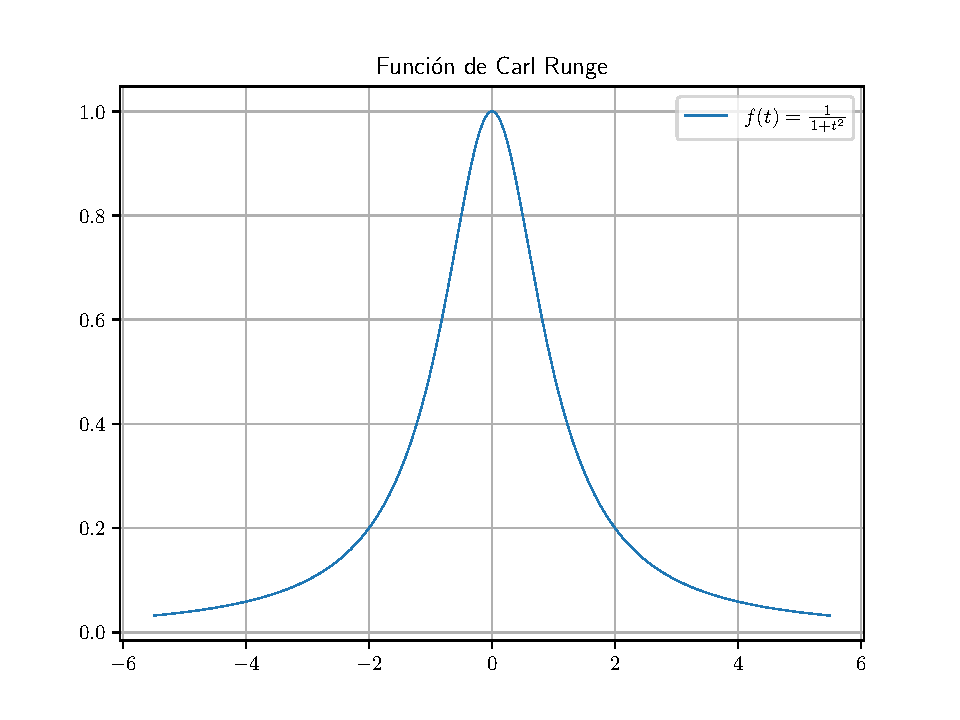
\includegraphics[width=.6\paperwidth]{p12}
        \end{figure}
    \end{solution}
\end{frame}

% \section{Pregunta N$^{\circ}$13\qquad Leon Alonzo Terrones Caccha}

\begin{frame}
    \begin{enumerate}\setcounter{enumi}{12}
        \item
            Demostrar que las funciones de Berstein para $n=3$ son l.i.
             
    \end{enumerate}

    \begin{solution}

    Sea la combinación lineal con $c_k\in\mathbb{R}:$
    \[\sum_{k=0}^{3}=c_{k}B_{k,3}(t)\]
    Por demostrar que $c_k=0$, $i\in[0.3]$
    \begin{align*}
        \sum_{k=0}^{3}=c_{k}B_{k,3}(t)&=\sum_{k=0}^{3}c_k\binom{3}{k}t^k(1-t)^{3-k}\\
        &=\sum_{k=0}^{3}{c_k\binom{3}{k}t^k\sum_{j=0}^{n-k}\binom{3-k}{j}{(-t)^{3-k-j}}}\\
        &=\sum_{j=0}^{3}{t^{n-j}\sum_{k=0}^{3-j}{c_k\binom{3}{k}\binom{3-k}{j}(-1)^{3-k-j}}}
    \end{align*}

    El cual es un polinomio de grado 3. Sean sus coeficientes $a_i$.
Para $j=0$, el coeficiente de $t^3$ es:
\begin{align*}
    a_{3}&=\sum_{k=0}^{3}{c_k\binom{3}{k}\binom{3-k}{0}(-1)^{3-k}}\\
    &=-c_0+3c_1-3c_2+c_3\\
    a_{2}&=\sum_{k=0}^{2}{c_k\binom{3}{k}\binom{3-k}{1}(-1)^{2-k}}\\
    &=3c_0-6c_1+3c_2\\
    a_{1}&=\sum_{k=0}^{2}{c_k\binom{3}{k}\binom{3-k}{1}(-1)^{2-k}}\\
    &=-3c_0+3c_1\\
    a_{0}&=\sum_{k=0}^{2}{c_k\binom{3}{k}\binom{3-k}{1}(-1)^{2-k}}\\
    &=c_0\\
\end{align*}


Al final se obtiene un sistema lineal en funcion del vector $c=(c_0,c_1,c_2,c_3)$. Debido a que $\{1,t,t^2,t^3\}$ es una base para los polinomios de grado 3 se tiene que $a_k=0$. Finalmente aplicando sustitución





    
    \begin{comment}
        \[
\begin{array}{cccccc}
x_0=0 & y_0=0 \\
    &     & 1 \\
x_1=1 & y_1=1 &             & \frac{\sqrt{3}-3}{6}\\
    &     & \frac{\sqrt{3}-1}{2}\\
x_2=3 & y_2=\sqrt{3}
\end{array}
\]
    \end{comment}

        
    \end{solution}
\end{frame}
\begin{frame}\transblindsvertical
	\frametitle{Referencias}
	%------------------------------------------------------------ 1
	\only<1>{
		\begin{itemize}
			\item Libros
			      \nocite{*}
			      \printbibliography[heading=none,keyword=book]
		\end{itemize}
	}
	%------------------------------------------------------------ 2
	\only<2>{
		\begin{itemize}
			\item Artículos científicos
			      \printbibliography[heading=none,keyword=paper]
		\end{itemize}
	}
	%------------------------------------------------------------ 3
	\only<3>{
		\begin{itemize}
			\item Sitios web
			      \printbibliography[heading=none,keyword=online]
		\end{itemize}
	}
\end{frame}

\end{document}